\documentclass[12pt]{article}
\usepackage{tabularx}
\usepackage{amsmath} 
\usepackage{graphicx}
\usepackage[margin=1in]{geometry}
\usepackage{cite}
\usepackage[final]{hyperref}
\hypersetup{
	colorlinks=true,      
	linkcolor=blue,       
	citecolor=blue,       
	filecolor=magenta,    
	urlcolor=blue         
}
\usepackage{blindtext}
\usepackage{amssymb}
\usepackage{esint}
\usepackage{tikz}
\usepackage{pgfplots}
\usepackage{gensymb}
\usetikzlibrary{datavisualization}
\usetikzlibrary{datavisualization.formats.functions}
\newcommand{\Prho}{.8}%
\newcommand{\Ptheta}{55}%
\newcommand{\Pphi}{60}%
\usepackage{tikz-3dplot}
\newcommand{\uvec}[1]{\boldsymbol{\hat{\textbf{#1}}}}
%++++++++++++++++++++++++++++++++++++++++
\usepackage{empheq}

\newcommand*\widefbox[1]{\fbox{\hspace{2em}#1\hspace{2em}}}

\begin{document}

\usetikzlibrary{scopes}
\def\iangle{35} % Angle of the inclined plane

\def\down{-90}
\def\arcr{0.5cm} % Radius of the arc used to indicate angles


\title{ECE 3030 - HW 4}
\author{Joshua Tensuan - jvt24}
\date{September 23, 2022}
\maketitle


\begin{enumerate}
	\item [4.1]
	We can use cylindrical coordinates for this problem where the $z$-axis is pointing into the page.
	From the symmetry of the setup, we can say that the magnetic field will only have a component in the polar $\phi$-direction.
	If we draw an Amperian concentric circle in the coaxial cable setup with radius $0<r<a$, we know that there will be no enclosed current.
	Thus, the line integral of the magnetic field in this region will be $0$.
	If we draw an Amperian concentric circle (orientation into the page) in the coaxial cable setup with radius $a<r<a+t$, we know that there will be an enclosed current given by $\iint \vec J \cdot d\vec A$.
	We can find $J$ by,
	\[J=I/A, \; A= \pi(a+t)^2-\pi a^2=2\pi a t + \pi t^2\]
	Thus,
	\[J=\frac{I}{2\pi a t + \pi t^2}\]
	Because we have a uniform current density,
	\[\iint \vec J \cdot d\vec A = J\cdot A = \frac{I}{2\pi a t + \pi t ^ 2}\left(\pi r^2-\pi a^2\right)=\frac{Ir^2}{2at + t^2}-\frac{Ia^2}{2at + t^2}\]
	Through Ampere's Law,
	\[\oint \vec B \cdot d\vec l =\mu_0 \iint \vec J \cdot d\vec A\]
	\[\to B_\phi\cdot 2\pi r = \mu_0\left(\frac{Ir^2}{2at + t^2}-\frac{Ia^2}{2at + t^2}\right)\]
	We then get a magnetic field in this region of,
	\[\to B_\phi = \mu_0\left(\frac{Ir}{2\pi\cdot(2at + t^2)}-\frac{Ia^2}{2\pi r\cdot (2at + t^2)}\right)\]
	Now, drawing an Amperian concentric circle (orientation into the page) in the coaxial cable with radius $a+t<r<b$, we know that the total current enclosed will be given by $I$.
	Thus, through Ampere's Law,
	\[\oint \vec B \cdot d\vec l = \mu_0\iint \vec J \cdot d\vec A\]
	\[\to B_\phi \cdot 2\pi r = \mu_0I\]
	We then get a magnetic field in this region of,
	\[B_\phi = \frac{\mu_0 I}{2\pi r}\]
	Now, drawing an Amperian concentric circle (orientation into the page) in the coaxial cable with radius $b < r < b+t$, we know that there will be an enclosed current given by $I+\iint \vec J \cdot dA$.
	We can find $J$ by,
	\[J=-I/A, \; A = \pi(b+t)^2-\pi b^2=2\pi b t + \pi t^2\]
	Thus,
	\[J = -\frac{I}{2\pi b t + \pi t^2}\]
	Because we have a uniform current density,
	\[\iint \vec J \cdot d\vec A = J \cdot A = -\frac{I}{2\pi b t + \pi t^2}(\pi r^2 - \pi b^2)=-\frac{Ir^2}{2bt+t^2}+\frac{Ib^2}{2bt + t^2}\]
	Through Ampere's Law,
	\[\oint \vec B \cdot d\vec l = \mu_0 I_{\mathrm{enc}}=\mu_0\left(I + \iint\vec J \cdot d\vec A\right)\]
	\[B_\phi \cdot (2\pi r)=\mu_0\left(I-\frac{Ir^2}{2bt+t^2}+\frac{Ib^2}{2bt+t^2}\right)\]
	This gives us a magnetic field in the region of,
	\[\to B_\phi =\mu_0I\left(\frac{1}{2\pi r}-\frac{r}{2\pi(2bt+t^2)}+\frac{b^2}{2\pi r(2bt+t^2)}\right)\]
	Drawing an Amperian concentric circle (orientation into the page) in the coaxial cable with radius $r>b+t$, we notice that $I_{\mathrm{enc}}=I-I=0$.
	Thus, there will be no magnetic field outside the coaxial cable.
	Thus, we have a total magnetic field of (note that $\hat \phi$ points in counterclockwise direction in plane of page)
	\[\boxed{\vec B=0, \; 0 < r < a}\]
	\[\boxed{\vec B=\mu_0\left(\frac{Ir}{2\pi\cdot(2at + t^2)}-\frac{Ia^2}{2\pi r\cdot (2at + t^2)}\right) \hat \phi, \; a < r < a+t}\]
	\[\boxed{\vec B = \frac{\mu_0 I}{2\pi r}\hat \phi, \; a+t < r < b}\]
	\[\boxed{\vec B =\mu_0I\left(\frac{1}{2\pi r}-\frac{r}{2\pi(2bt+t^2)}+\frac{b^2}{2\pi r(2bt+t^2)}\right)\hat \phi, \; b < r < b+t}\]
	\[\boxed{\vec B=0, \; r>b+t}\]
	The plot is then given by,

	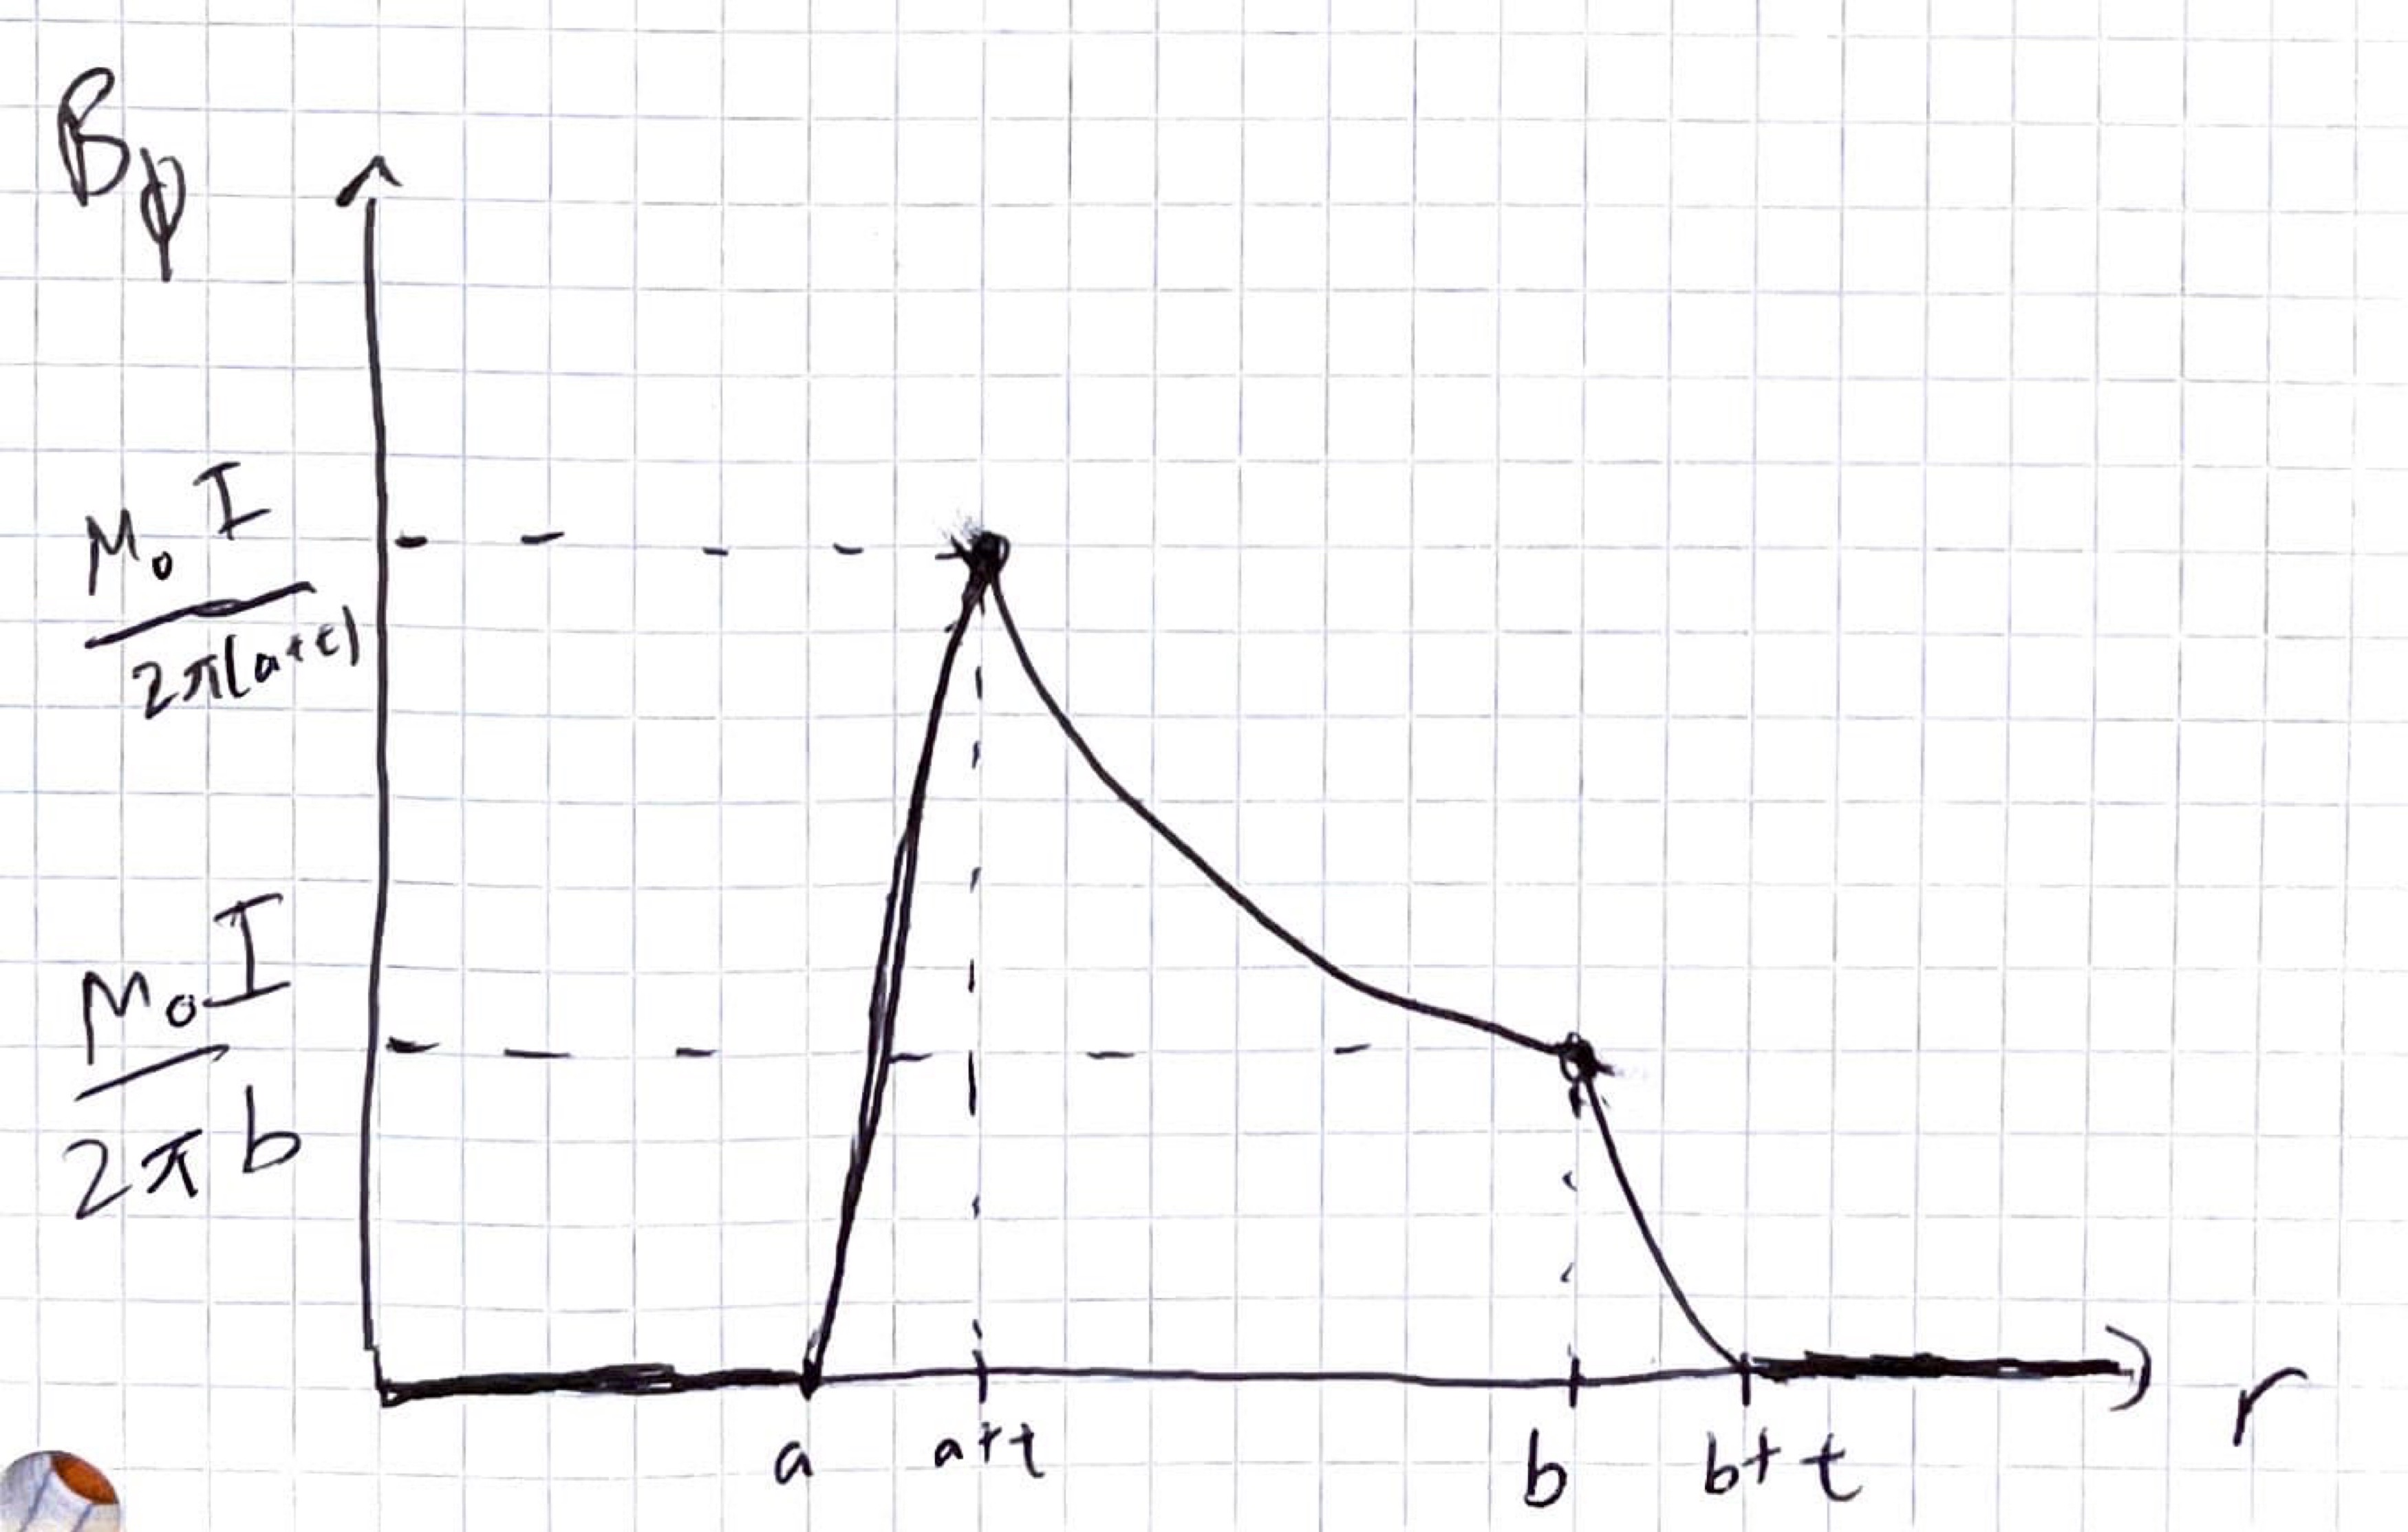
\includegraphics[width = 5in]{images/IMG_3794.JPG}

	\item [4.2]
	\begin{enumerate}
		\item [a.]
		Let the $z$-axis correspond to the axis of the solenoid.
		By symmetry, we know that there will only be a magnetic field contribution in the $z$-direction.
		Ampere's Law tells us that,
		\[\oint \vec H \cdot d\vec l = \iint \vec J \cdot d\vec A\]
		We know that far away from the solenoid, the $H$-field is $0$.
		Thus, if we form any Amperian loop outside the solenoid, the current enclosed will be $0$.
		Thus, the $H$-field outside the solenoid will be $0$.
		If we form an Amperian rectangle with one side outside the solenoid, and the other inside, with the loop perpendicularly piercing the solenoid, we know that the only contribution to the line integral will be the side of the rectangle along the $z$-axis inside the solenoid.
		$\iint \vec J \cdot d\vec A$ is then given by, the current multiplied by the number of windings through the Amperian rectangle.
		Thus,
		\[H_zL = NI \to H = nI\hat z\]
		We notice that this is independent of the material inside the solenoid.
		We defined $\vec B$ to be,
		\[\vec B=\mu_0(\vec H + \vec M)=\mu_0\vec H(1+\chi_m)=\mu \vec H\]
		We notice that for the region $r<a$, $\mu=\mu$, while for $a<r<b$, $\mu=\mu_0$.
		Thus,
		\[\vec B = \begin{cases}
			\mu nI \hat z & r < a \\ 
			\mu_0 nI \hat z & a < r < b	
		\end{cases}\]
		We can solve for $\vec M$ through trivial algebra,
		\[\vec M = \vec B - \mu_0 \vec H\]
		Then,
		\[\vec M = \begin{cases}
			(\mu nI-\mu_0 nI) \hat z & r < a \\ 
			(\mu_0 nI-\mu_0nI) \hat z & a < r < b	
		\end{cases}\]
		\[\vec M = \begin{cases}
			(\mu nI-\mu_0 nI) \hat z & r < a \\ 
			0 & a < r < b	
		\end{cases}\]
		Thus,
		\[\boxed{\vec H = nI \hat z, \; 0 < r < b}\]
		\[\boxed{\vec B = \begin{cases}
			\mu nI \hat z & r < a \\ 
			\mu_0 nI \hat z & a < r < b	
		\end{cases}}\]
		\[\boxed{\vec M = \begin{cases}
			(\mu nI-\mu_0 nI) \hat z & r < a \\ 
			0 & a < r < b	
		\end{cases}}\]

		\item [b.]
		Finding the magnetic flux $\lambda$ through the solenoid,
		\[\lambda=\iint \vec B \cdot d\vec A\]
		We can split this into two regions, $r<a$ and $a<r<b$.
		Because the magnetic fields are constant in these two regions, the magnetic flux is trivial to calculate as,
		\[\lambda = B_1A_1 + B_2A_2\]
		where the subscript 1 refers to the region $r<a$ and subscript 2 refers to the region $a<r<b$.
		\[\lambda = \mu n I \pi a^2 + \mu_0 n I (\pi b^2-\pi a^2)\]
		\[\lambda = \pi nI((\mu-\mu_0) a^2 + \mu_0 b^2)\]
		The $\lambda$ without the rod is given by $\pi n I \mu_0 b^2$.
		Since $\mu>\mu_0$, we can say that inserting the rod in, increases the magnetic flux in the solenoid.
		\[\boxed{\lambda = \pi nI((\mu-\mu_0) a^2 + \mu_0 b^2)}\]
		\[\boxed{\text{Inserting rod/magnetic material increases magnetic flux.}}\]

	\end{enumerate}

	\item [4.3]
	\begin{enumerate}
		\item [a.]
		Solving Laplace's Equation, we know that $A_z$ will only have a dependence on $r$ and $\varphi$ by symmetry.
		Thus,
		\[\frac{1}{r}\frac{\partial}{\partial r}\left(r\frac{\partial A_z}{\partial r}\right)+\frac{1}{r^2}\frac{\partial^2 A_z}{\partial \varphi^2}=0\]
		\[\to \frac{\partial}{\partial r}\left(r\frac{\partial A_z}{\partial r}\right)=-\frac{1}{r}\frac{\partial^2 A_z}{\partial \varphi^2}\]
		Using the separation of variables technique, we know that $A_z$ will have both a part dependent on $r$ and part dependent on $\varphi$.
		Thus, we can write $A_z$ as, $A_z=u(r)v(\varphi)+C$.
		Then,
		\[\frac{\partial}{\partial r}\left(ru'v\right)=-\frac{1}{r}uv''\]
		\[\to u'v + ru''v=-\frac{1}{r}uv''\]
		Separating the variables,
		\[\to ru'v + r^2u''v=uv''\]
		\[\to r\left(\frac{u'}{u}+r\frac{u''}{u}\right)=\frac{v''}{v}\]
		If we take the partial derivative of both sides with respect to $\varphi$, we find that the left-side is only dependent on $r$, and thus the partial derivative will be equal to $0$.
		Thus, $v''/v=C$.
		Similarly, the left-hand side of the equation will equal the same constant $C$
		Starting with,
		\[\frac{v''}{v}=C \to v''=Cv\]
		Trivially, any linear combination of $\sin(\varphi)$ and $\cos(\varphi)$ functions will satisfy this differential equation.
		In order to match the current distribution, let's set $v=A\sin(\varphi)$.
		Taking the left-hand side of the equation now,
		\[r\left(\frac{u'}{u}+r\frac{u''}{u}\right)=C\]
		\[\left(\frac{u'}{u}+r\frac{u''}{u}\right)=\frac{C}{r}\]
		\[\to ru'' + u' - \frac{Cu}{r}=0\]
		Through trial and error, we find that both $u=Br$ and $u=B/r$,
		Far away from the system, we want $u\to 0$.
		Thus, outside of the system, we should take the solution $B/r$.
		Meanwhile, inside the system, we want $u$ to not diverge.
		Thus, inside the system, we should take the solution $Br$.
		Combining both solutions via $A_z=u(r)v(\varphi)+C$, we end up with our trial solutions of,
		\[\boxed{\begin{cases}
			A_z^{\mathrm{in}}(r,\varphi) = Ar\sin(\varphi)+C \\ 
			A_z^{\mathrm{out}}(r,\varphi)=\frac{B}{r}\sin(\varphi)+D
		\end{cases}}\]

		\item [b.]
		From $\nabla \cdot \vec H=0$, we can conclude that the component of the magnetic field normal to the boundary is continuous.
		This is trivial to derive if we form a small test surface right across the boundary.
		Additionally, from Ampere's Law, we know that,
		\[\oint \vec H \cdot d\vec s = \iint \vec J \cdot d\vec A\]
		If we form a small Amperian loop around the boundary, we find that,
		\[L(H_{2\parallel}-H_{1\parallel})=KL\to H_{2\parallel}-H_{1\parallel}=K\]
		where $K$ is the surface current density through the Amperian loop.
		We know that $\vec H$ is related to $\vec A$ by, $\mu_0 \vec H = \nabla \times \vec A$.
		For a vector with only a $z$-component in cylindrical coordinates,
		\[\nabla \times \vec A = \frac{1}{r}\frac{\partial A_z}{\partial \varphi}\hat r-\frac{\partial A_z}{\partial r}\hat \varphi\]
		Thus,
		\[\vec H =\frac{1}{\mu_0}\nabla \times \vec A = \frac{1}{\mu_0}\left(\frac{1}{r}\frac{\partial A_z}{\partial \varphi}\hat r - \frac{\partial A_z}{\partial r}\hat \varphi\right)\]
		For this system, the radial component of $\vec H$ corresponds to the perpendicular component of $\vec H$ and the $\varphi$-component of $\vec H$ corresponds to the parallel component of $\vec H$.
		Enforcing the tangential $\vec H$-field boundary condition,
		\[\frac{1}{\mu_0}\frac{1}{r}\frac{\partial A_z^{\mathrm{in}}(r=a)}{\partial \varphi}=\frac{1}{\mu_0}\frac{1}{r}\frac{\partial A_z^{\mathrm{out}}(r=a)}{\partial \varphi}\]
		\[\to \frac{\partial A_z^{\mathrm{in}}(r=a)}{\partial \varphi}=\frac{\partial A_z^{\mathrm{out}}(r=a)}{\partial \varphi}\]
		Enforcing the parallel $\vec H$-field boundary condition,
		\[\frac{1}{\mu_0}\left(\frac{\partial A_z^{\mathrm{in}}(r=a)}{\partial r}-\frac{\partial A_z^{\mathrm{out}}(r=a)}{\partial r}\right)=K_0\sin(\varphi)\]
		\[\to \frac{\partial A_z^{\mathrm{in}}(r=a)}{\partial r}-\frac{\partial A_z^{\mathrm{out}}(r=a)}{\partial r}=\mu_0K_0\sin(\varphi)\]
		We know that far away from the system, the $A$ should approach $0$.
		Thus,
		\[\lim_{r\to\infty}A_z^{\mathrm{out}}(r) = 0\]
		Additionally, we require that the vector potential be continuous across the boundary.
		Thus,
		\[A_z^{\mathrm{in}}(r=a)=A_z^{\mathrm{out}}(r=a)\]
		This gives us 4 boundary conditions with 4 undetermined coefficients from part a.
		\[\boxed{\begin{cases}
			\frac{\partial A_z^{\mathrm{in}}(r=a)}{\partial \varphi}=\frac{\partial A_z^{\mathrm{out}}(r=a)}{\partial \varphi} \\ 
			\frac{\partial A_z^{\mathrm{in}}(r=a)}{\partial r}-\frac{\partial A_z^{\mathrm{out}}(r=a)}{\partial r}=\mu_0K_0\sin(\varphi) \\ 
			\lim_{r\to\infty}A_z^{\mathrm{out}}(r) = 0 \\ 
			A_z^{\mathrm{in}}(r=a)=A_z^{\mathrm{out}}(r=a)
		\end{cases}}\]

		\item [c.]
		From the third boundary condition, we know that,
		\[\lim_{r\to\infty}A_z^{\mathrm{out}}(r) = D = 0\]
		Thus, $D=0$.
		Using the first boundary condition,
		\[\frac{\partial A_z^{\mathrm{in}}}{\partial \varphi}=Ar\cos(\varphi)\]
		\[\frac{\partial A_z^{\mathrm{out}}}{\partial \varphi}=\frac{B}{r}\cos(\varphi)\]
		Setting these two equal to each other at $r=a$, using the first boundary condition,
		\[Aa=\frac{B}{a}\to B=Aa^2\]
		Using the second boundary condition,
		\[\frac{\partial A_z^{\mathrm{in}}}{\partial r}=A\sin(\varphi)\]
		\[\frac{\partial A_z^{\mathrm{out}}}{\partial r}=-\frac{B}{r^2}\sin(\varphi)\]
		Substituting these into the second boundary condition with $r=a$,
		\[A\sin(\varphi)+\frac{B}{a^2}\sin(\varphi)=\mu_0K_0\sin(\varphi)\]
		\[A+\frac{B}{a^2}=\mu_0K_0\]
		Substituting in $B=Aa^2$ as we derived earlier,
		\[2A=\mu_0K_0\to A = \frac{\mu_0K_0}{2}\]
		Similarly,
		\[B=Aa^2=a^2\frac{\mu_0K_0}{2}\]
		Utilizing the last boundary condition,
		\[A_z^{\mathrm{in}}(r=a) = a\frac{\mu_0K_0}{2}\sin(\varphi)+C\]
		\[A_z^{\mathrm{out}}(r=a) = a\frac{\mu_0K_0}{2}\sin(\varphi)+D\]
		Setting these two equal to each other, we find that, $C=D=0$.
		Thus,
		\[\boxed{\begin{cases}
			A = \mu_0K_0/2 \\
			B = a^2(\mu_0K_0/2) \\
			C = 0 \\ 
			D = 0	
		\end{cases}}\]
		Substituting these in,
		\[\boxed{A_z = \begin{cases}
			r\mu_0K_0\sin(\varphi)/2 & 0 < r \leq a \\ 
			a^2\mu_0K_0\sin(\varphi)/2r & r \geq a
		\end{cases}}\]

		\item [d.]
		As derived previously, we found that,
		\[\vec H = \frac{1}{\mu_0}\nabla \times \vec A = \frac{1}{\mu_0}\left(\frac{1}{r}\frac{\partial A_z}{\partial \varphi}\hat r - \frac{\partial A_z}{\partial r}\hat \varphi\right)\]
		First, finding $\vec H$ in the region of $0< r \leq a$,
		\[\vec H_{\mathrm{in}}=\frac{1}{\mu_0}\left(\frac{1}{r}\cdot\left(\frac{r\mu_0K_0\cos(\varphi)}{2}\right)\hat r - \left(\frac{\mu_0K_0\sin(\varphi)}{2}\right)\hat \varphi\right)\]
		\[\vec H_{\mathrm{in}} =\frac{K_0\cos(\varphi)}{2}\hat r  - \frac{K_0\sin(\varphi)}{2}\hat \varphi\]
		Similarly, finding $\vec H$ in the region of $r\geq a$,
		\[\vec H_{\mathrm{out}} = \frac{1}{\mu_0}\left(\frac{1}{r}\cdot\left(\frac{a^2\mu_0K_0\cos(\varphi)}{2r}\right)\hat r-\left(-\frac{a^2\mu_0K_0\sin(\varphi)}{2r^2}\right)\hat \varphi\right)\]
		\[\vec H_{\mathrm{out}}=\frac{a^2K_0\cos(\varphi)}{2r^2}\hat r+\frac{a^2K_0\sin(\varphi)}{2r^2}\hat \varphi\]
		Compiling all this,
		\[\boxed{\vec H  = \begin{cases}
			\frac{K_0\cos(\varphi)}{2}\hat r  - \frac{K_0\sin(\varphi)}{2}\hat \varphi & 0 < r \leq a \\ 
			\frac{a^2K_0\cos(\varphi)}{2r^2}\hat r+\frac{a^2K_0\sin(\varphi)}{2r^2}\hat \varphi & r \geq a
		\end{cases}}\]

		\item [e.]
		The sketch of the magnetic field is given below,

		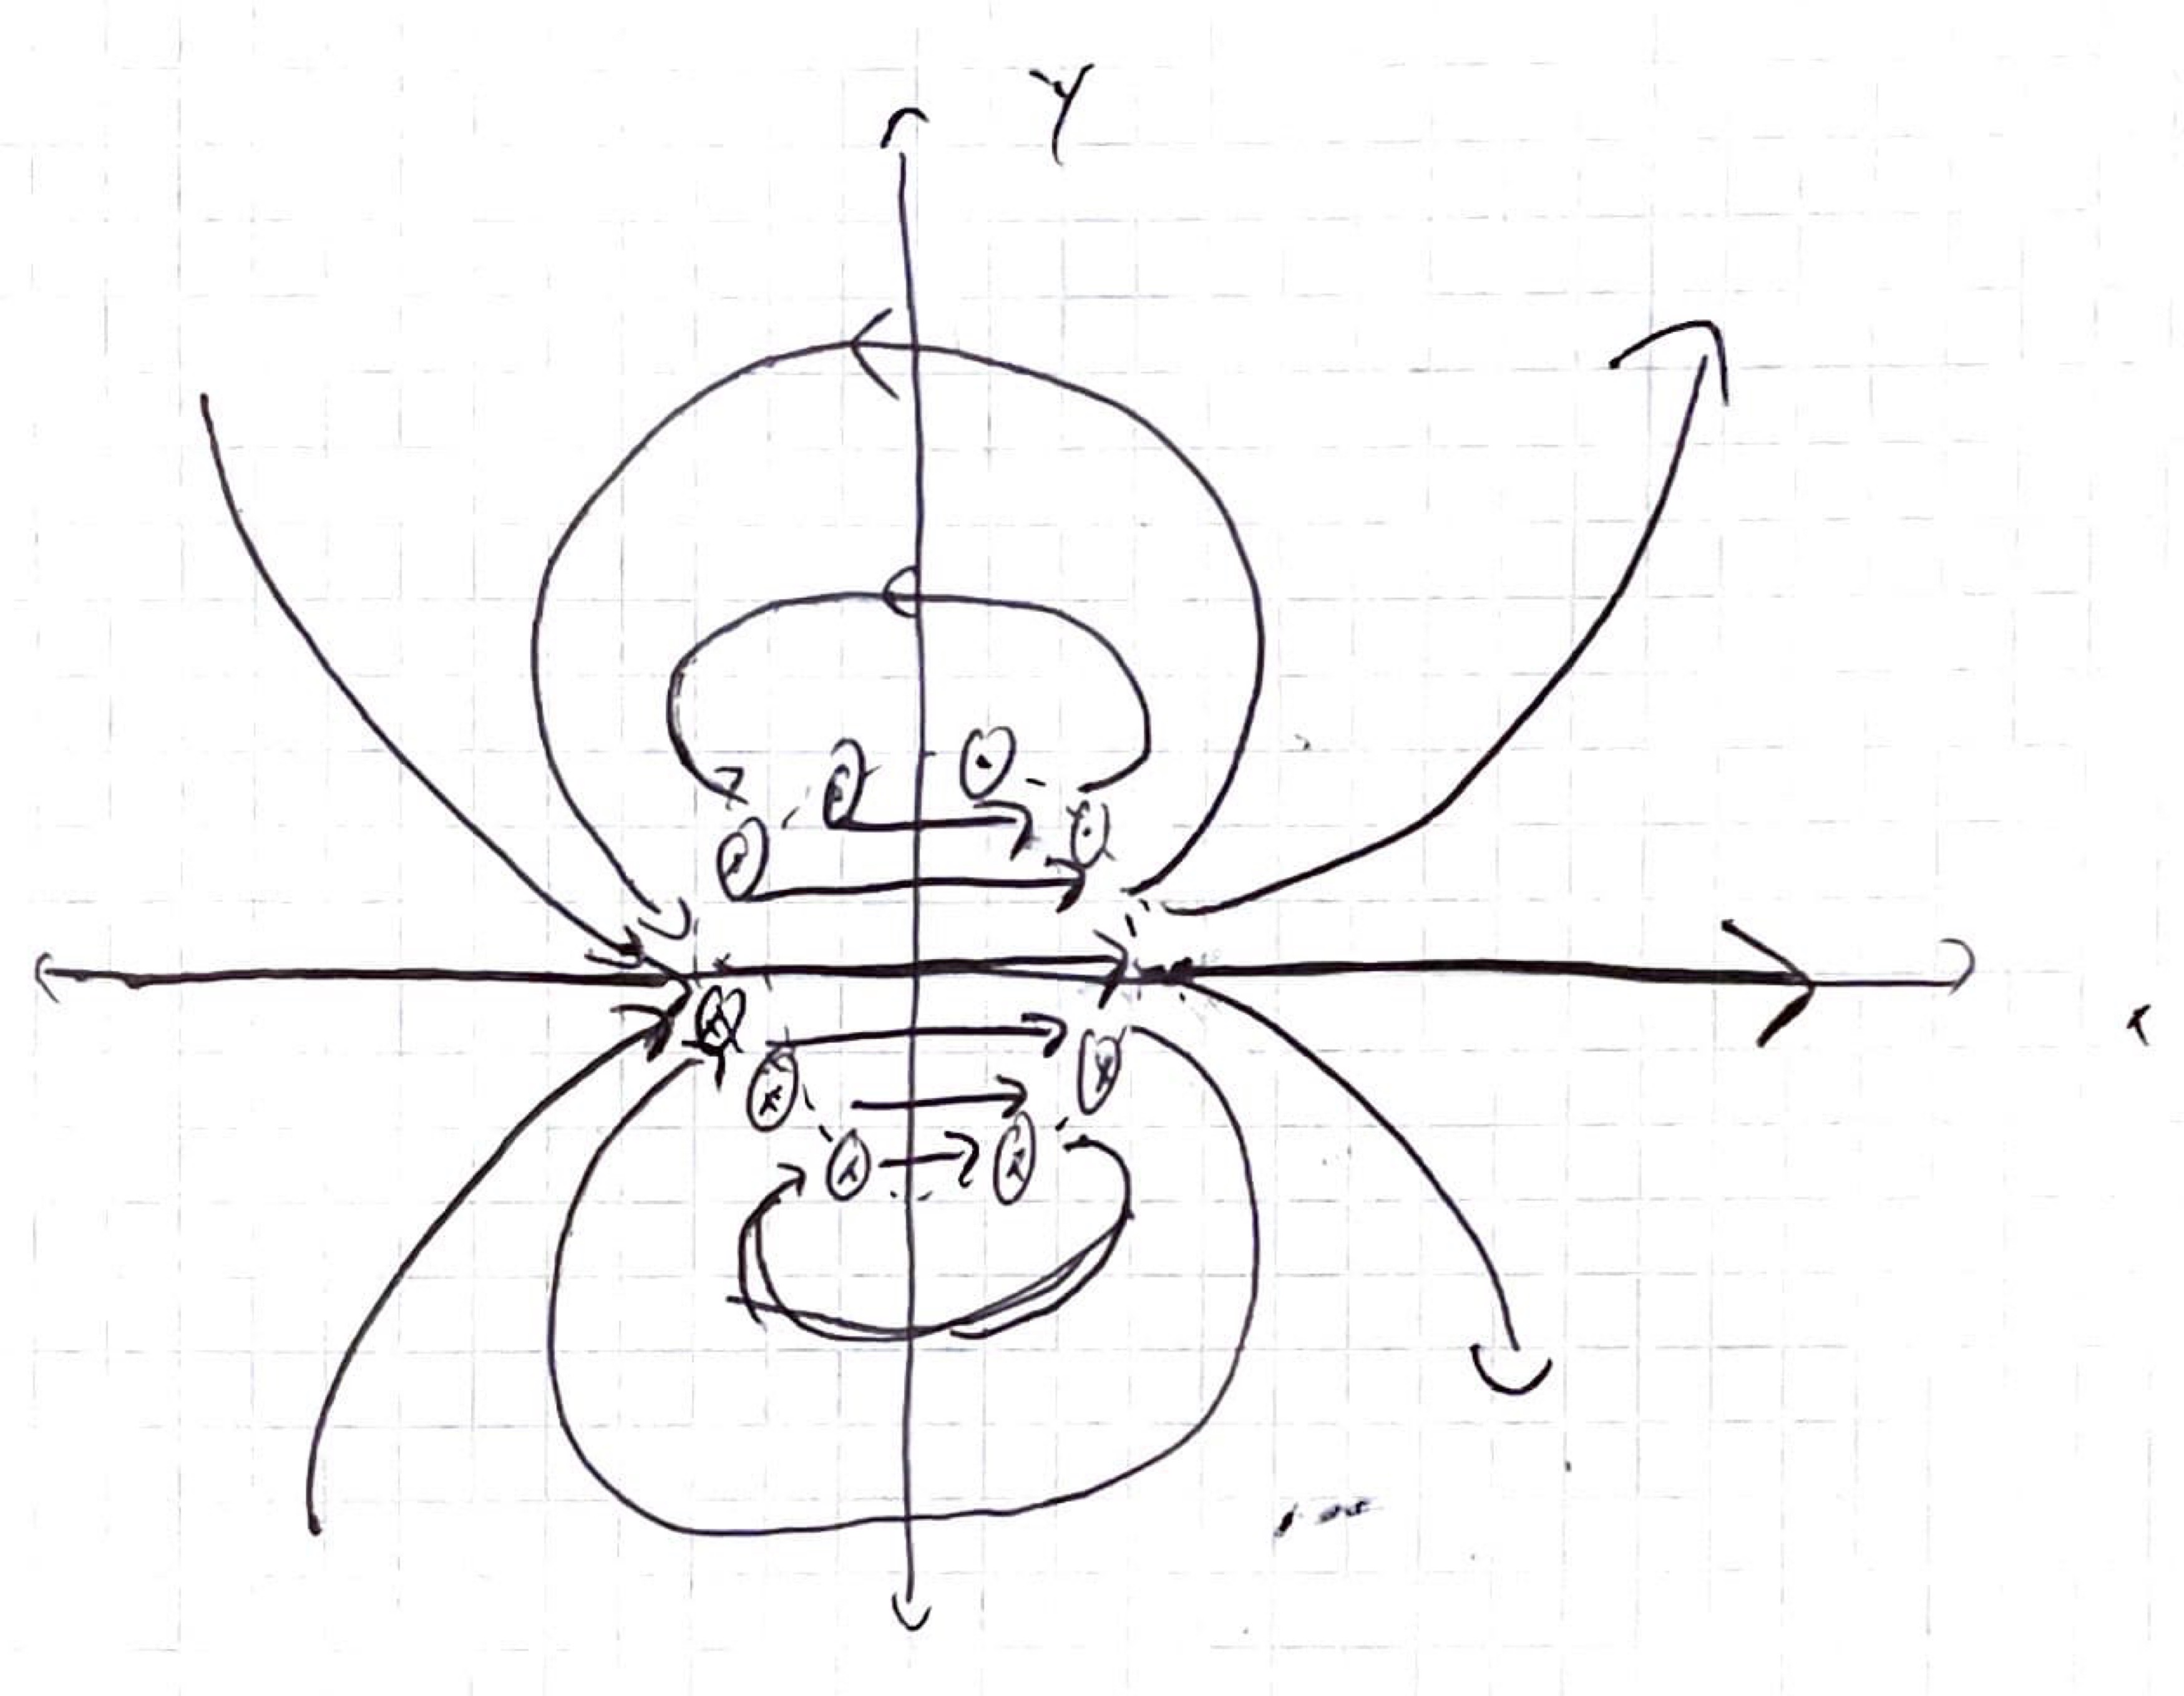
\includegraphics[width = 5in]{images/IMG_3795.JPG}







	\end{enumerate}

	\item [4.4]
	\begin{enumerate}
		\item [a.]
		From Faraday's Law, we know that,
		\[\oint \vec E \cdot d\vec s = -\frac{\partial}{\partial t}\iint \vec B \cdot d\vec A\]
		We know that $\oint \vec E \cdot d\vec s = -2iR$.
		Substituting this in,
		\[2iR = \frac{\partial}{\partial t}\iint \vec B \cdot d\vec A\]
		Solving the flux integral,
		\[\iint \vec B \cdot d\vec A = \int_0^{0.1}\int_0^{0.3}\cos(\omega t-ky)\: dx \: dy=0.3 \cdot \int_0^{0.1}\cos(\omega t - ky)\: dy\]
		\[\iint \vec B \cdot d\vec A =0.3 \cdot \left[-\frac{1}{k}\sin(\omega t - ky)\right]_{y=0}^{0.1}\]
		\[=0.3 \cdot \left(\frac{1}{k}\sin(\omega t)-\frac{1}{k}\sin(\omega t - 0.1k)\right)\]
		Taking the partial derivative with respect to time,
		\[\frac{\partial}{\partial t}\iint \vec B \cdot d\vec A = 0.3 \cdot \left(\frac{\omega}{k}\cos(\omega t)-\frac{\omega}{k}\cos(\omega t - 0.1k)\right)\]
		\[\frac{\partial}{\partial t}\iint \vec B \cdot d\vec A = 0.3 \frac{\omega}{k} \left(\cos(\omega t)-\cos(\omega t - 0.1k)\right)\]
		Substituting this into our expression from Faraday's Law,
		\[2iR = 0.3 \frac{\omega}{k} \left(\cos(\omega t)-\cos(\omega t - 0.1k)\right)\]
		\[i = \frac{1}{2R}\cdot0.3 \frac{\omega}{k} \left(\cos(\omega t)-\cos(\omega t - 0.1k)\right)\]
		Substituing in $R=10 \Omega$,
		\[i(t) = 0.015 \frac{\omega}{k} \left(\cos(\omega t)-\cos(\omega t - 0.1k)\right)\]
		\[\boxed{i(t) = \left[0.015 \frac{\omega}{k} \left(\cos(\omega t)-\cos(\omega t - 0.1k)\right)\right] \mathrm{A}}\]

		\item [b.]
		From Faraday's Law, we know that,
		\[\oint \vec E \cdot d\vec s = -\frac{\partial}{\partial t}\iint \vec B \cdot dvec A\]
		We know that $\oint \vec E \cdot d\vec s = -iR$ by Ohm's Law.
		Substituting this in,
		\[iR = \frac{\partial}{\partial t}\iint \vec B \cdot d\vec A\]
		Solving the flux integral,
		\[\iint \vec B \cdot d\vec A = \int_0^{0.35(1-\cos(\omega t))}\int_0^{0.2}\cos(\omega t)\: dy \: dx\]
		\[\iint \vec B \cdot d\vec A = 0.2 \cdot (0.35(1-\cos(\omega t)))\cdot \cos(\omega t)\]
		Simplifying this expression,
		\[\iint \vec B \cdot d\vec A = 0.07 \cdot(\cos(\omega t)-\cos^2(\omega t))\]
		Taking the partial derivative with respect to time,
		\[\frac{\partial}{\partial t}\iint \vec B \cdot d\vec A = -0.07\omega\sin(\omega t) + 2\cdot 0.07 \cdot \omega \cos(\omega t)\sin(\omega t)\]
		\[\frac{\partial}{\partial t}\iint \vec B \cdot d\vec A = -0.07\omega\sin(\omega t) + 0.14 \cdot \omega \cos(\omega t)\sin(\omega t)\]
		Substituting this into our expression from Faraday's Law,
		\[iR = -0.07\omega\sin(\omega t) + 0.14 \cdot \omega \cos(\omega t)\sin(\omega t)\]
		\[i(t) = \frac{1}{R}\left[-0.07\omega\sin(\omega t) + 0.14 \cdot \omega \cos(\omega t)\sin(\omega t)\right]\]
		Substituting in $R=1\Omega$,
		\[i(t) = \left[-0.07\omega\sin(\omega t) + 0.14 \cdot \omega \cos(\omega t)\sin(\omega t)\right]\]
		\[\boxed{i(t) = \left[-0.07\omega\sin(\omega t) + 0.14 \cdot \omega \cos(\omega t)\sin(\omega t)\right]\mathrm{A}}\]

		\item [c.]
		In effect, the rod will act as another resistor and will adjust our equation for Faraday's Law.
		We can find the effective resistance of the rod by,
		\[R= \frac{L}{\sigma A}\]
		Substituting in $L=0.2 \: \mathrm{m}$,
		\[R = \frac{0.2}{\sigma A}\]
		Then, we find that, adding up resistances because they are in series,
		\[\oint \vec E \cdot d\vec s = -i\left(R + \frac{0.2}{\sigma A}\right)\]
		Thus, if we go back to our expression with Faraday's Law from part b,
		\[i\left(R + \frac{0.2}{\sigma A}\right)=-0.07\omega\sin(\omega t) + 0.14 \cdot \omega \cos(\omega t)\sin(\omega t)\]
		Substituting in $R=1\:\Omega$,
		\[i(t)=\frac{1}{1+(0.2/\sigma A)}\cdot\left(-0.07\omega\sin(\omega t) + 0.14 \cdot \omega \cos(\omega t)\sin(\omega t)\right)\]
		\[\boxed{i(t)=\left[\frac{1}{1+(0.2/\sigma A)}\cdot\left(-0.07\omega\sin(\omega t) + 0.14 \cdot \omega \cos(\omega t)\sin(\omega t)\right)\right] \mathrm{A}}\]
		In other words, the resulting current will be smaller from our answer in part b by some factor of the added resistance.
	\end{enumerate}



	
	
	
\end{enumerate}

		

\end{document}
